% Created 2019-10-30 Wed 16:07
% Intended LaTeX compiler: pdflatex
\documentclass{scrartcl}
\usepackage[utf8]{inputenc}
\usepackage[T1]{fontenc}
\usepackage{graphicx}
\usepackage{grffile}
\usepackage{longtable}
\usepackage{wrapfig}
\usepackage{rotating}
\usepackage[normalem]{ulem}
\usepackage{amsmath}
\usepackage{textcomp}
\usepackage{amssymb}
\usepackage{capt-of}
\usepackage{hyperref}
\hypersetup{colorlinks,linkcolor=black,urlcolor=blue}
\usepackage{textpos}
\usepackage{textgreek}
\usepackage[version=4]{mhchem}
\usepackage{chemfig}
\usepackage{siunitx}
\usepackage{gensymb}
\usepackage[usenames,dvipsnames]{xcolor}
\usepackage[T1]{fontenc}
\usepackage{lmodern}
\usepackage{verbatim}
\usepackage{tikz}
\usepackage{wasysym}
\usetikzlibrary{shapes.geometric,arrows,decorations.pathmorphing,backgrounds,positioning,fit,petri}
\author{Matthew Henderson, PhD, FCACB}
\date{\today}
\title{Lysosomal Storage Disease}
\hypersetup{
 pdfauthor={Matthew Henderson, PhD, FCACB},
 pdftitle={Lysosomal Storage Disease},
 pdfkeywords={},
 pdfsubject={},
 pdfcreator={Emacs 26.1 (Org mode 9.1.9)}, 
 pdflang={English}}
\begin{document}

\maketitle
\tableofcontents


\tikzstyle{chemical} = [rectangle, rounded corners, text width=5em, minimum height=1em,text centered, draw=black, fill=none]
\tikzstyle{hardware} = [rectangle, rounded corners, text width=5em, minimum height=1em,text centered, draw=black, fill=gray!30]
\tikzstyle{ms} = [rectangle, rounded corners, text width=5em, minimum height=1em,text centered, draw=orange, fill=none]
\tikzstyle{msw} = [rectangle, rounded corners, text width=7em, minimum height=1em,text centered, draw=orange, fill=none]
\tikzstyle{label} = [rectangle,text width=8em, minimum height=1em, text centered, draw=none, fill=none]
\tikzstyle{hl} = [rectangle, rounded corners, text width=5em, minimum height=1em,text centered, draw=black, fill=red!30]
\tikzstyle{box} = [rectangle, rounded corners, text width=5em, minimum height=5em,text centered, draw=black, fill=none]
\tikzstyle{arrow} = [thick,->,>=stealth]
\tikzstyle{hl-arrow} = [ultra thick,->,>=stealth,draw=red]


\section{Sphingolipid Synthesis}
\label{sec:org6b1e6ee}
\subsection{Introduction}
\label{sec:orgf96697c}
\begin{enumerate}
\item Sphingolipids
\label{sec:orgfecfdc4}

\begin{itemize}
\item Found in all mammalian cell membranes
\item Plasma lipoproteins
\item Structural role
\item Modulate numerous biological functions
\begin{itemize}
\item apoptosis
\end{itemize}
\item named after the Sphinx because of their enigmatic nature\ldots{}
\end{itemize}

\item Sphingosine and Ceramide
\label{sec:org41dee53}

\begin{itemize}
\item long chain sphingolipid base
\item N-acylated by a variety of fatty acids
\end{itemize}
\centering

\definesubmol{x}{-[7,.3]-[1,.3]}
\definesubmol{y}{-[:+30,.3]=[:-30,.3]}
\definesubmol{a}{-[1,.3](=[2,.3]O)!x!x!x!x!x!x!x!x!x!x!x}
\chemfig{OH!x([2,.5]<HN)-[7,.3](-[6,.3]OH)-[1,.3]=[7,.3]-[1,.3]!x!x!x!x!x!x}
\chemfig{OH!x([2,.5]<HN!a)-[7,.3](-[6,.3]OH)-[1,.3]=[7,.3]-[1,.3]!x!x!x!x!x!x}
%%\chemfig{!b}



\item Biosynthesis
\label{sec:org7e7b04d}

\begin{enumerate}
\item ER
\label{sec:org5f64e5e}
\begin{itemize}
\item condensation of serine and palmitoyl-CoA \(\to\) sphinganine
\item N-acylation \(\to\) ceramide
\end{itemize}

\item Golgi
\label{sec:org1cd6231}
\begin{itemize}
\item stepwise addition of monosaccharides
\begin{itemize}
\item sphingomyelin
\item glucosylceramide
\item glycosphingolipids
\item gangliosides
\end{itemize}
\end{itemize}
\end{enumerate}

\item Sphingolipid Structure
\label{sec:orgc5db135}

\begin{figure}[htbp]
\centering
\includegraphics[width=\textwidth]{./sphingolipid_synthesis/figures/Sphingolipids_general_structures.png}
\caption[Sphingolipid Structure]{\label{fig:orgba703de}
Sphingolipid Structure}
\end{figure}

\item Sphingolipid Biosynthesis
\label{sec:org2af3f8a}

\begin{figure}[htbp]
\centering
\includegraphics[width=0.6\textwidth]{./sphingolipid_synthesis/figures/synthesis.png}
\caption[Sphingolipid Biosynthesis]{\label{fig:orgcb42f9d}
Sphingolipid Biosynthesis}
\end{figure}
\end{enumerate}

\subsection{Disorders of Sphingolipid Synthesis}
\label{sec:org1ca97df}
\begin{enumerate}
\item Serine Palmitoyltransferase (Subunit 1 or 2) Deficiency
\label{sec:orgc6a1302}

\begin{itemize}
\item Defect in first step of sphingolipid biosynthesis
\item Major cause of dominant Hereditary Sensory and Autonomic Neuropathies (HSAN1).
\begin{itemize}
\item Late onset (2-4th decade)
\item peripheral sensory neuropathy
\item distal sensory loss
\item ulcerative mutilations
\item hypohydrosis
\item there is a more severe early onset form
\end{itemize}
\item Accumulation of sphingoid bases \(\to\) pathology
\item mutations in serine palmitoyltransferase (SPCTLC1 or 2) alter
substrate specificity
\begin{itemize}
\item serine \(\to\) alanine and glycine
\end{itemize}
\item Elevated plasma 1-deoxy-sphingamine, 1-deoxy-methyl-sphingamine, 1-deoxy-ceramindes
\item Trial of serine supplementation
\end{itemize}

\item Ceramide Synthases 1 and 2
\label{sec:orgca21d63}

\begin{itemize}
\item Six human ceramide synthases
\begin{itemize}
\item tissue and acyl-CoA substrate specificity
\item Neurological CERS1 \&2
\begin{description}
\item[{CER1}] Myoclonic epilepsy, cognitive decline
\begin{itemize}
\item Decreased C18-ceramide in cultured fibroblasts
\end{itemize}
\item[{CER2}] Myoclonic epilepsy
\begin{itemize}
\item Decreased VLC-ceramide in cultured fibroblasts
\end{itemize}
\end{description}
\item Dermatologic CERS3
\begin{description}
\item[{CER3}] Ichthyosis
\begin{itemize}
\item Lack of VLC-ceramides in skin and fibroblasts
\end{itemize}
\end{description}
\end{itemize}
\end{itemize}


\item Fatty Acid 2-Hydroxylase
\label{sec:org4ce6488}

\begin{itemize}
\item spastic paraplegia
\begin{itemize}
\item fatty acid hydroxylase associated neurodegeneration (FAHN)
\end{itemize}
\item 38 patients, most in present in childhood
\item slowly progressing
\begin{itemize}
\item spastic paraplegia
\item dysarthria
\item mild cognitive decline
\item dystonia
\end{itemize}

\item Insufficiency production of 2-hydroxy-galactosphingolipids
\begin{itemize}
\item required in myelin
\item increase with brain development
\end{itemize}

\item Decreased hydroxylated sphingomyelin in cultured cells
\end{itemize}

\item GM3 Synthase Deficiency
\label{sec:org991d673}

\begin{itemize}
\item Autosomal recessive infantile-onset epilepsy
\begin{itemize}
\item Amish epilepsy syndrome
\end{itemize}
\item In first year \(\to\) generalized tonic-clonic seizures
\begin{itemize}
\item profound developmental stagnation and regression
\item salt and pepper syndrome
\begin{itemize}
\item hyper and hypo-pigmented skin maculae
\item facial dysmorphism scoliosis
\item intellectual disability
\item seizures
\item choreoathetosis
\item spasticity
\end{itemize}
\end{itemize}

\item lack of GM3, GD3 and higher gangliosides, and increased
lactosylceramide and Gb4 levels in plasma and cultured cells
\end{itemize}


\item GM2/GD2 Synthase Deficiency
\label{sec:org1d9d90a}

\begin{itemize}
\item Mutations of B4GALNT1
\item SPG26, a slowly progressive complex hereditary spastic paraplegia
with mild to moderate cognitive impairment.

\item Cultured fibroblasts of patients have shown decreased GM2 levels
with an increase of its precursor, GM3.
\end{itemize}

\item Non-lysosomal β-Glucosidase Deficiency
\label{sec:orgad76341}

\begin{itemize}
\item GBA2 is a membrane-associated protein localised at the ER and Golgi
\begin{itemize}
\item hydrolyse glucosylceramide to ceramide and glucose.
\end{itemize}
\item GBA2 is distinct from the lysosomal acid \(\beta\)-glucosidase GBA1 deficient in Gaucher disease
\item hereditary (complex) spastic paraplegia locus SPG46.
\item Starting in childhood marked spasticity in lower extremities with
progressive gait disturbances
\begin{itemize}
\item later, ataxia and other cerebellar signs
\end{itemize}
\end{itemize}

\item Ceramide Synthase 3 and ULFA \(\omega\)-Hydroxylase
\label{sec:orgac08a24}

\begin{itemize}
\item ceramides in skin maintain skin barrier homeostasis, prevent water
loss and protect against microbial infections
\item Autosomal recessive congenital ichthyosis (ARCI) is a heterogeneous
group of disorders of epidermal cornification
\item 9 causative genes have been identified including CERS3 and CYP4F22

\item[{CERS3}] ichthyosis
\begin{itemize}
\item lack of ceramides with VLCFA in cultured fibroblasts
\end{itemize}
\item[{CYP4F22}] ichthyosis
\begin{itemize}
\item lack of ceramides with ULCFA in cultured fibroblasts
\end{itemize}
\end{itemize}

\item Classification
\label{sec:org353fd33}

\begin{enumerate}
\item Primarily nervous system involvement
\label{sec:orgc70bd29}
\begin{itemize}
\item Serine palmitoyltransferase - peripheral sensory neuropathy
\item Ceramide synthase 1 - myoclonic epilepsy
\item Ceramide synthase 2 - myoclonic epilepsy
\item Fatty Acid 2-hydroxylase - SPG35
\item Nonlysosomal β-Glucosidase - SPG46
\item GM3 Synthase Deficiency - Amish infantile epilepsy
\item GM2/GD2 Synthase Deficiency - SPG26
\end{itemize}


\item Primarily skin involvement
\label{sec:org0aa9a6f}
\begin{itemize}
\item Ceramide synthase 3 - Ichthyosis
\item ULCFA \(\omega\)-hydrolase - Ichthyosis
\end{itemize}
\end{enumerate}
\end{enumerate}

\section{Gaucher}
\label{sec:orgd5b93ca}
\subsection{Introduction}
\label{sec:org81b4be9}

\begin{enumerate}
\item Gaucher
\label{sec:org6310561}
\begin{itemize}
\item Caused by accumulation of glucosylceramide (glucocerebroside).
\item Defect in \(\beta\)-glucocerebrosidase
\begin{itemize}
\item Extremely rare SAP-C deficiency
\end{itemize}
\item Most common LSD
\begin{itemize}
\item 1:40,000 to 1:50,000 live births
\end{itemize}
\item Three types:
\begin{description}
\item[{Type 1}] No neurological symptoms
\item[{Type 2}] Acute neuronopathic
\item[{Type 3}] Sub-acute or chronic neuronopathic
\end{description}
\item Type 1 disease is common in Western Europe, the Americas and Israel
\item In many other countries neuronopathic forms of Gaucher disease predominate
\end{itemize}

\item Sphingolipid degradation
\label{sec:org1536c0b}

\begin{figure}[htbp]
\centering
\includegraphics[width=0.6\textwidth]{./gaucher/figures/sl_degradation.png}
\caption{\label{fig:org8548e86}
Sphingolipid degradation}
\end{figure}

\item Glucocerebroside: the Gaucher lipid
\label{sec:org8fafbbe}

\begin{figure}[htbp]
\centering
\includegraphics[width=0.5\textwidth]{./gaucher/figures/glucocerebroside.png}
\caption{\label{fig:org325ac18}
Glucocerebroside}
\end{figure}

\item Glucocerebrosidase
\label{sec:org4737409}


\begin{figure}[htbp]
\centering
\includegraphics[width=0.5\textwidth]{./gaucher/figures/glucocerebrosidase.png}
\caption{\label{fig:org1fb5d97}
\(\beta\)-glucocerebrosidase}
\end{figure}

\begin{itemize}
\item Located in the lumen of lysosomes
\item LIMP-2 is responsible for mannose 6-phosphate receptor independent
lysosomal targeting of \(\beta\)-glucocerebrosidase
\end{itemize}

\item Genetics
\label{sec:org0d76244}
\begin{itemize}
\item Autosomal recessive, GBA gene
\item Most of the >300 disease alleles in Gaucher disease are missense
mutations
\begin{itemize}
\item result in \(\beta\)-glucocerebrosidase with decreased catalytic
function and/or stability.
\end{itemize}
\item A variety of complex mutations/rearrangements also causes Gaucher
disease:
\begin{itemize}
\item missense mutations, frame shift mutations, splicing mutations,
deletions, gene fusions with the pseudogene, examples of gene
conversions, and total deletions.
\end{itemize}
\item genotype/phenotype correlations exist for:
\begin{itemize}
\item type 1 disease (N370S)
\item types 2 and 3 (L444P)
\end{itemize}
\item within these categories there is variable penetrance and
expressivity between individuals and ethnic groups.
\end{itemize}
\end{enumerate}


\subsection{Clinical Findings}
\label{sec:orgf9020ac}
\begin{enumerate}
\item Clinical Presentation
\label{sec:orge1712be}

\begin{table}[htbp]
\caption{\label{tab:org6c6c647}
Gaucher Clinical Variants}
\centering
\begin{tabular}{llll}
 & Type 1 & Type 2 & Type 3\\
\hline
Onset & Infant/Child/Adult & 3-6 months & Childhood\\
Neurodegeneration & Absent & \texttt{++++} & \texttt{++} \(\to\) \texttt{++++}\\
Survival & 6 - 80+ years & < 2 years & 2nd - 4th decade\\
Splenomegaly & \texttt{++++} & \texttt{++} & \texttt{++}\\
Hepatomegaly & \texttt{++} & \texttt{++} & \texttt{+}\\
Fractures, bone crises & \texttt{+} & - & \texttt{+}\\
Enrichment & Ashkenazi & None & Norrbottnian\\
 &  &  & Swedish\\
\end{tabular}
\end{table}

\item Clinical Presentation
\label{sec:orgfeb4626}

\begin{figure}[htbp]
\centering
\includegraphics[width=\textwidth]{./gaucher/figures/variants.png}
\caption{\label{fig:org3458815}
Gaucher Clinical Variants}
\end{figure}

= * Parkinson Disease, ** Myoclonic Seizures =
\item Gaucher type 1
\label{sec:orgf616eae}
\begin{itemize}
\item Clinical manifestations of Gaucher type 1 are linked to macrophages
engorged with glucosylceramide.

\item An undefined mechanism results in:
\begin{itemize}
\item enlargement and dysfunction of the liver and spleen
\item displacement of normal bone marrow by storage cells
\item osteoclastic-osteoblastic imbalances
\begin{itemize}
\item subsequent damage leading to bone infarctions and fractures.
\end{itemize}
\item Occasionally, involvement of other organs (e.g. lung) contributes
to the overall clinical picture.
\item Hypermetabolism and cachexia can be present
\item Thrombocytopenia is the most common peripheral blood abnormality
\end{itemize}

\item Neurological manifestations include:
\begin{itemize}
\item a high incidence of Parkinsonism
\item spinal cord compression
\item nerve root compression
\item polyneuropathy.
\end{itemize}
\end{itemize}

\item Gaucher type 2
\label{sec:orgd861109}
\begin{itemize}
\item Type 2 is the rarer of the two classic neuronopathic variants1
\item early infantile onset of acute neuronopathic disease
\item progressing rapidly to death before age 2 years

\begin{itemize}
\item retroflexion of the neck
\item developmental delay, poor weight gain,
\item protuberant abdomen due to hepatosplenomegaly
\item Bulbar signs are prominent including:
\begin{itemize}
\item convergent squint,
\item ocular paresis,
\item trismus,
\item dysphagia
\end{itemize}
\end{itemize}

\item The perinatal-lethal subtype is the most severe form of Gaucher
disease.

\begin{itemize}
\item leads to death in utero or within hours to days after
birth
\end{itemize}
\end{itemize}

\item Gaucher type 3
\label{sec:orgd6328ad}
\begin{itemize}
\item type 3 disease has a later onset, with slower progression of
neurologic manifestations and variable degrees of systemic
involvement.
\item phenotype in type 3 Gaucher disease is considerably more
heterogeneous than that in type 2.

\item onset of symptoms occurs later, and neurologic involvement
progresses more slowly

\item includes abnormalities in:
\begin{itemize}
\item eye movements
\item seizures
\item intellectual deterioration.
\end{itemize}

\item The same systemic manifestations occur as in type 1 disease.
\begin{itemize}
\item many type 3 patients may be incorrectly classified as type 1 when
first seen
\end{itemize}
\end{itemize}

\item Gaucher type 3
\label{sec:org9937953}
\begin{enumerate}
\item Gaucher type 3a
\label{sec:org5b68ccd}
\begin{itemize}
\item progressive myoclonus and dementia
\end{itemize}

\item Gaucher type 3b
\label{sec:org349044c}
\begin{itemize}
\item horizontal supranuclear gaze palsy without other major
neurologic signs
\item aggressive systemic disease
\end{itemize}

\item Gaucher type 3c
\label{sec:org94ae5dc}
\begin{itemize}
\item present in late childhood or later
\item only mild visceral signs of classic Gaucher disease
\item distinguishing clinical signs include:
\begin{itemize}
\item impaired horizontal ocular saccades
\item corneal opacities
\item cardiac/aortic valvular calcification
\end{itemize}
\end{itemize}
\end{enumerate}
\end{enumerate}

\subsection{Laboratory Investigations}
\label{sec:orga10473b}
\begin{enumerate}
\item Gaucher Cells
\label{sec:org3f44409}

\begin{figure}[htbp]
\centering
\includegraphics[width=0.8\textwidth]{./gaucher/figures/Gaucher_Cells_with_Fibrillar_Appearing_Cytoplasm.jpg}
\caption{\label{fig:org66d7181}
Gaucher Cells}
\end{figure}

\item Biochemistry
\label{sec:orge7a7e92}
\begin{enumerate}
\item Enzyme Assay
\label{sec:orgc7903ac}
\begin{itemize}
\item assay of the \(\beta\)-glucocerebrosidase activity in any nucleated cell
\begin{itemize}
\item the enzyme does not normally occur in plasma/serum or erythrocytes
\end{itemize}
\item Glucocerebrosidase activity in:
\begin{itemize}
\item peripheral blood lymphocytes/leukocytes
\item dried blood spots
\end{itemize}
\item 4MU-\(\beta\)-D--glucopyranoside substrate
\end{itemize}

\item Monitoring
\label{sec:orgac949c9}
\begin{itemize}
\item chitotriosidase, chemokine CLL18/PARK, glucosylsphingosine
\end{itemize}
\end{enumerate}

\item Molecular
\label{sec:org2571a07}

\begin{itemize}
\item GBA gene sequencing, >300 disease alleles
\item Patients homozygous for the L444P mutation have severe visceral
disease, highly predisposed to the development of CNS disease.
\item The N370S mutant enzyme appears to preclude the development of classical CNS disease of Gaucher disease.
\item The D409H mutation manifests a characteristic phenotype:
\begin{itemize}
\item including cardiac calcification, oculomotor apraxia, and corneal opacities.
\end{itemize}
\end{itemize}
\end{enumerate}

\subsection{Treatment}
\label{sec:orgc0bb8f6}
\begin{enumerate}
\item Bone marrow transplantation
\label{sec:org54d9e63}
\begin{itemize}
\item Curative for Type 1
\begin{itemize}
\item Suggests hematopoietic gene therapy
\end{itemize}
\item High risk of mortality
\end{itemize}
\item ERT
\label{sec:org52328f6}
\begin{itemize}
\item treats: hematological, visceral, and bony disease
\begin{itemize}
\item not cerebral disease
\end{itemize}
\item macrophages have a mannose receptor
\begin{itemize}
\item glucocerebrosidase glycoprotein modified to expose terminal mannose
\end{itemize}
\item 1991, Ceredase (algucerase) - human placenta
\item 1994, Cerezyme (imiglucerase) - CHO cells
\item 2010, VPRIV (velaglucerase) - human fibroblasts
\end{itemize}

\item Substrate reduction therapy
\label{sec:org3a0ae96}
\begin{itemize}
\item ceramide glucoyltransferase inhibitor
\begin{itemize}
\item N-butyldeoxynojirimycin (miglustate)
\item eliglustat tartrate
\end{itemize}
\item Chaperone to stabilize - missense mutation
\begin{itemize}
\item isofagomine
\end{itemize}
\end{itemize}
\end{enumerate}

\section{Niemann-Pick}
\label{sec:org5d8cdb1}
\subsection{Introduction}
\label{sec:org619707a}

\begin{enumerate}
\item Niemann-Pick Disease
\label{sec:orgc8a9f2c}
\begin{itemize}
\item There are two distinct diseases called Niemann-Pick
\begin{itemize}
\item Types A and B (acid sphingomyelinase deficiency)
\item Type C (cholesterol recycling)
\end{itemize}
\end{itemize}

\item Niemann-Pick A \& B
\label{sec:org9b92dfd}
\begin{itemize}
\item Incidence of Niemann-Pick A among Ashkenazi Jews \textasciitilde{} 1:40,000.
\item Incidence of both Niemann–Pick A and B in all other populations \textasciitilde{} 1:250,000.
\item Niemann-Pick Type A and B are caused by deficiency of acid sphingomyelinase (ASM).
\begin{itemize}
\item sphingomyelinase is required to metabolize sphingomyelin.
\item results in progressive accumulation of sphingomyelin in systemic organs
\begin{itemize}
\item brain accumulation in neuronal forms
\end{itemize}
\item There is growing evidence that NPA \& NPB represent opposite ends of a continuum.
\begin{itemize}
\item NPA generally have little or no ASM production (less than 1\% of normal).
\item NPB have approximately 10\% of normal level of ASM.
\end{itemize}
\end{itemize}
\end{itemize}

\item Sphingomyelin and Sphingomyelinase
\label{sec:org6ebf8ad}

\begin{figure}[htbp]
\centering
\includegraphics[width=0.8\textwidth]{./niemann_pick/figures/sphingomyelin.png}
\caption{\label{fig:org360e3c4}
Sphingomyelin}
\end{figure}

\begin{figure}[htbp]
\centering
\includegraphics[width=0.8\textwidth]{./niemann_pick/figures/sphingomyelinase.png}
\caption{\label{fig:orgd3763f2}
Sphingomyelinase}
\end{figure}


\item Sphingolipid degradation
\label{sec:org2abaf29}

\begin{figure}[htbp]
\centering
\includegraphics[width=0.6\textwidth]{./niemann_pick/figures/sl_degradation.png}
\caption{\label{fig:orgc3dab82}
Sphingolipid degradation}
\end{figure}

\item Niemann-Pick C
\label{sec:org8e96ce5}
\begin{itemize}
\item a fatal, neuro-degenerative disease that affects \textasciitilde{} 1:150,000
\begin{itemize}
\item sometimes referred to as Childhood Alzheimer’s
\item extremely heterogeneous
\item biochemically, genetically and clinically distinct from Niemann-Pick A and B.
\end{itemize}
\item Accumulation of unesterified cholesterol, sphingomyelin, glycolipids in systemic organs
\item GM2 and GM3 accumulate in brain
\begin{itemize}
\item no increase in cholesterol
\end{itemize}
\item NPC has two sub types NP-C1 (95\%) and NP-C2 (5\%)
\end{itemize}

\item Niemann-Pick C
\label{sec:org099c039}

\begin{itemize}
\item LDL cholesterol enters cells via endocytosis at the LDL receptor.
\item delivered to the late-stage endosomes and lysosomes
\item hydrolyzed and released as free cholesterol.
\item Unesterified cholesterol is transported to the plasma membrane and the ER for recycling.

\item In NP-C, the LDL-cholesterol is trapped in lysosomes
\end{itemize}

\begin{figure}[htbp]
\centering
\includegraphics[width=0.8\textwidth]{./niemann_pick/figures/cholesterol1.jpg}
\caption{\label{fig:orgbed2a8a}
Cholesterol Transport}
\end{figure}


\item NPC1 \& NPC2
\label{sec:org72cca02}

\begin{figure}[htbp]
\centering
\includegraphics[width=0.65\textwidth]{./niemann_pick/figures/Niemann-Pick-C-Brown-and-Goldstein.png}
\caption{\label{fig:org9ac4e4e}
NPC1 \& NPC2}
\end{figure}

\begin{itemize}
\item NPC1 is a lysosomal membrane protein involved in transport in the endosomal-lysosomal system
\item NPC2 acts in cooperation with the NPC1
\item The disruption of transport results in accumulation of cholesterol and glycolipids in lysosomes.
\end{itemize}

\item Lysosomal Protein Trafficking
\label{sec:org270ed08}

\begin{figure}[htbp]
\centering
\includegraphics[width=0.65\textwidth]{./niemann_pick/figures/lysosome_trafficking.jpeg}
\caption{\label{fig:orgcef5b9a}
Lysosomal protein trafficking receptors}
\end{figure}

\begin{itemize}
\item lysosomal trafficking of acid sphingomyelinase is mediated by sortilin and mannose 6-phosphate receptor.
\item MPR alone is sufficient to transport NPC2 to the endo/lysosomal compartment
\item Sorting of LMPs from Golgi/PM to endosomal system is mediated by
signals in the cytosolic domain
\end{itemize}

\item Genetics
\label{sec:orgcbbe4c0}

\begin{enumerate}
\item Niemann-Pick A \& B
\label{sec:org788bd22}
\begin{itemize}
\item Mutations in SMPD1
\item Good phenotype-genotype correlation
\end{itemize}
\item Niemann-Pick C
\label{sec:orga0d487d}
\begin{itemize}
\item Autosomal recessive inheritance,
\item Mutations in NPC1 (95\%) and NPC2 (5\%)
\end{itemize}
\end{enumerate}
\end{enumerate}

\subsection{Clinical Findings}
\label{sec:orgc83281c}

\begin{enumerate}
\item Niemann-Pick A \& B symptoms
\label{sec:org89db66c}

\begin{enumerate}
\item Niemann-Pick A symptoms
\label{sec:org5de822c}
\begin{itemize}
\item hepatosplenomegaly by age 3 months
\item Failure to thrive
\item Psychomotor regression at age 1
\begin{itemize}
\item progressive loss of abilities – mental and physical
\end{itemize}
\item Interstitial lung disease resulting in lung infections and lung failure
\item Cherry-red spot identified with eye examination (100\%)
\end{itemize}

\item Niemann-Pick B symptoms
\label{sec:org0be0848}
\begin{itemize}
\item Symptoms outlined under NPA (but less severe)
\item Thrombocytopenia
\item Short stature
\item Cherry-red spot identified with eye examination (50\%)
\end{itemize}
\end{enumerate}

\item Niemann-Pick C symptoms
\label{sec:org7c81d0b}

\begin{itemize}
\item onset of the disease can happen at any age.
\begin{itemize}
\item often school age children.
\item also adults
\end{itemize}

\item Symptoms may include:
\begin{itemize}
\item Jaundice at birth or shortly afterwards
\item Hepatosplenomegaly
\item Vertical supranuclear gaze palzy
\item Ataxia
\item Dystonia
\item Dysarthria
\item Cognitive dysfunction/dementia
\item Cataplexy
\item Tremors accompanying movement
\item Seizures
\item Dysphagia
\end{itemize}
\end{itemize}

\begin{enumerate}
\item Definitions:
\label{sec:org36cdfd6}
\begin{itemize}
\item Vertical Supranuclear Gaze Palzy: Difficulty with Upward \& Downward Eye Movement
\item Ataxia: Unsteadiness with Gait, Clumsiness or Walking
\item Dystonia:  neurological movement disorder syndrome in which sustained or repetitive muscle contractions result in twisting and repetitive movements or abnormal fixed postures
\item Dysarthria: Slurred Irregular Speech
\item Cognitive Dysfunction/Dementia: Learning Difficulties \& Progressive Intellectual Decline
\item Cataplexy: Sudden Loss of Muscle Tone Which May Lead to Unexpected Falls
\item Dysphagia:Swallowing Problems
\item Thrombocytopenia: low number of platelets
\end{itemize}
\end{enumerate}

\item Niemann-Pick C neurological forms
\label{sec:org7a5c5eb}

\small
\begin{itemize}
\item Classification by neurological form is widely used
\item correlation between age at neurological onset and course of disease
and lifespan has been established
\end{itemize}

\begin{enumerate}
\item Early infantile
\label{sec:org14257fb}
\begin{itemize}
\item pre-existing hepatosplenomegaly
\item delay in motor milestones 9m-2yrs
\item survival <6 years
\end{itemize}

\item Late-infantile
\label{sec:org2f89d0b}
\begin{itemize}
\item classic NPC, 60-70\% of cases
\item language delay
\item Ataxia, 3-5 yrs
\item Cognitive dysfunction, 6-12 yrs
\end{itemize}

\item Adult
\label{sec:org5729565}
\begin{itemize}
\item diagnosis 15->60yrs.
\item insidious presentation
\item ataxia, dystonia, dysarthria, movement disorders
\item variable cognitive dysfunction
\item Vertical gaze palzy common
\end{itemize}
\end{enumerate}
\end{enumerate}

\subsection{Laboratory Investigations}
\label{sec:org79d6d87}
\begin{enumerate}
\item Newborn Screening
\label{sec:orgf8bb295}
\begin{itemize}
\item New York state is conducting a pilot newborn screening program for four lysosomal storage disorders.
\item Pompe, Gaucher, Niemann-Pick A/B, Fabry, and MPS 1

\item 4 years, 65,605 infants participated, representing an overall consent rate of 73\%.
\begin{itemize}
\item Sixty-nine infants were screen-positive.
\item Twenty-three were confirmed true positives, all of whom were predicted to have late-onset phenotypes.
\item Six of the 69 currently have undetermined disease status.
\end{itemize}
\end{itemize}

\item Biomarkers: oxysterols
\label{sec:org48ac1fa}

\begin{itemize}
\item Plasma oxysterols
\begin{itemize}
\item oxysterols cholestane-3\(\beta\), 5\(\alpha\), 6\(\beta\)-triol
\item 7-ketocholesterol
\end{itemize}
\end{itemize}



\begin{figure}[htbp]
\centering
\includegraphics[width=0.7\textwidth]{./niemann_pick/figures/biomarkers.jpg}
\caption{\label{fig:orgc2baae5}
Klinke, G. Clin Biochem 2015}
\end{figure}

\item Biomarkers: lysosphingomylin
\label{sec:org0c821e5}

\begin{itemize}
\item Plasma and DBS
\begin{itemize}
\item lysosphingomylin
\item lysosphingomylin-509
\end{itemize}
\end{itemize}

\begin{figure}[htbp]
\centering
\includegraphics[width=0.8\textwidth]{./niemann_pick/figures/biomarkersII.jpg}
\caption{\label{fig:orgf6571b1}
Kuckar, L. Anal Biochem. 2017}
\end{figure}

\item Enzymology: Niemann-Pick A \& B
\label{sec:orgdc7ef32}

\begin{itemize}
\item Deficient ASM activity in leukocytes or cultured cells.
\begin{itemize}
\item use of native or radio-labelled substrate preferred to fluorescent substrate
\begin{itemize}
\item 6-hexadecanoylamino-4-methylumbelliferyl-phosphorylcholine
\item Does not detect Q292K mutation
\end{itemize}
\end{itemize}
\end{itemize}

\item Pathology: Niemann-Pick A \& B
\label{sec:org59ebd0f}

\begin{figure}[htbp]
\centering
\includegraphics[width=0.45\textwidth]{./niemann_pick/figures/foam_cells.png}
\caption{\label{fig:org200d0b7}
Foam cells in bone marrow}
\end{figure}

\item Niemann-Pick C
\label{sec:org595c67e}
\begin{itemize}
\item Filipin test
\begin{itemize}
\item Streptomyces filipinensis - anti-fungal
\item culture fibroblasts in an LDL-enriched medium
\item pathognomonic free cholesterol accumulation in lysosomes
\item fluorescence microscopy after filipin staining
\item unequivocal results in \textasciitilde{} 85\% of patients
\end{itemize}
\end{itemize}

\begin{figure}[htbp]
\centering
\includegraphics[width=0.5\textwidth]{./niemann_pick/figures/filipin.png}
\caption{\label{fig:org3f483cb}
Filipin staining (red:filipin, green:CellMask)}
\end{figure}
\end{enumerate}

\subsection{Treatment}
\label{sec:orgff8234d}
\begin{enumerate}
\item Treatment: Niemann-Pick A\&B
\label{sec:org842edd9}
\begin{itemize}
\item No approved treatments
\item Olipudase alfa, a recombinant human acid sphingomyelinase (ASM), is
an enzyme replacement therapy for the treatment of nonneurologic
manifestations of acid sphingomyelinase deficiency (ASMD).
\item ongoing, open-label, long-term study (NCT02004704) assessed safety
and efficacy of olipudase alfa following 30 months of treatment in
five adult patients with ASMD.
\item There were no deaths, serious or severe events, or discontinuations
during 30 months of treatment.
\item Chitotriosidase in serum and lyso-sphingomyelin in dried blood spots
decreased with olipudase alfa treatment
\end{itemize}

\item Treatment: Niemann-Pick C
\label{sec:orgcffa734}
\begin{itemize}
\item substrate reduction therapy
\begin{itemize}
\item miglustat approved for treatment of neurological manifestations
\item miglustat is an iminosugar, a synthetic analogue of D-glucose
\end{itemize}
\end{itemize}
\end{enumerate}

\section{GM1 \& GM2 Gangliosidoses}
\label{sec:orga9c09cf}
\subsection{Introduction}
\label{sec:orgb20fcda}

\begin{enumerate}
\item Sphingolipid degradation
\label{sec:org3819e1a}

\begin{figure}[htbp]
\centering
\includegraphics[width=0.6\textwidth]{./GM1_2/figures/sl_degradation.png}
\caption{\label{fig:orgabd4641}
Sphingolipid degradation}
\end{figure}

\item GM1 Gangliosidosis
\label{sec:org8c86e62}
\begin{itemize}
\item Defect in \(\beta\)-gangliosidase
\item GM1 ganglioside accumulates in the brain and visera
\item Infantile, juvenile and adult forms
\begin{itemize}
\item Residual enzyme function
\item Devastating degenerative disease
\end{itemize}
\item GM1 gangliosidosis of all types is estimated to occur in 1:100,000 - 300,000
\end{itemize}

\begin{enumerate}
\item MPS IVB - Morquio B
\label{sec:orged2135a}
\begin{itemize}
\item Clinically indistinguishable from MPS IVA
\begin{itemize}
\item skeletal changes, including short stature and skeletal dysplasia.
\item normal intelligence
\end{itemize}
\item The prevalence of MPS IVB has been reported as 1:250,000 - 1,000,000
\end{itemize}
\end{enumerate}


\item \(\beta\)-galactosidase
\label{sec:org5912042}
\begin{figure}[htbp]
\centering
\includegraphics[width=0.7\textwidth]{./GM1_2/figures/bgalatosidase.png}
\caption{\label{fig:org5287606}
\(\beta\)-galactosidase}
\end{figure}


\item Lysosomal multi-enzyme complex
\label{sec:org657afa7}

\begin{itemize}
\item \(\beta\)-galactosidase forms a heterotrimeric complex with:
\begin{itemize}
\item cathepsin A/PPCA : CTSA
\item neuraminidase: NEU1
\end{itemize}

\item \(\downarrow\) cathepsin A \(\to\) 2\degree  deficiency of NEU1
\begin{itemize}
\item ML-1 (sialidosis)
\end{itemize}
\end{itemize}

of the LMC and the CSER, and that become deregulated in case of
single or combined enzyme deficiencies in sialidosis, GM1 and
GS. CMA, chaperone mediated autophagy; CSER, cell surface elastin
receptor; EBP, elastin binding protein; ECM, extracellular matrix;
LM, lysosomal membrane; LMC, lysosomal multienzyme complex; PM,
plasma membrane
\begin{center}
\includegraphics[width=\textwidth]{./GM1_2/figures/lmc.jpg}
\label{org57d9985}
\end{center}

\item GM2 Gangliosidosis
\label{sec:org97636c0}
\begin{itemize}
\item Three genetic and biochemical subtypes
\begin{itemize}
\item Tay-Sachs disease
\item Sandhoff disease
\item GM2 activator deficiency
\end{itemize}
\item Impaired lysosomal catabolism of GM2 ganglioside.
\item GM2 storage in neurons in Tay-Sachs and Sandhoff
\begin{itemize}
\item Sandhoff \(\uparrow\) asialo-GM2 in brain, globoside and oligosacarides in viseral organs
\end{itemize}
\item Progressive cerebral degeneration
\item Prior to population-based carrier screening the incidence of TSD was \textasciitilde{}1:3600 Ashkenazi Jewish births.
\begin{itemize}
\item Incidence of TSD in the Ashkenazi Jewish population in North America \(\downarrow\) > 90\%
\end{itemize}
\item Eastern Quebec founder mutation
\end{itemize}


\item GM2 ganglioside storage diseases
\label{sec:org6ac333e}

\begin{center}
\begin{tabular}{llrl}
Disorder & Onset & Death (y) & Enzyme\\
\hline
Tay-Sachs disease & 3-6 months & 2-4 & Hex A\\
Sandhoff disease & 3-6 months & 2-4 & Hex A\&B\\
AB variant & 3-6 months &  & Activator\\
Juvenile GM 2 gangliosidosis & 2-6 years & 5-15 & Hex A\\
Adult GM 2 gangliosidosis & 2 yrs-adult & Variable & Hex A\\
\end{tabular}
\end{center}


\item Lysosomal \(\beta\)-Hexosaminidase enzymes
\label{sec:org64bfa13}

\begin{itemize}
\item Functional lysosomal \(\beta\)-hexosaminidase enzymes are dimeric.
\item Three isozymes are produced through the combination of \(\alpha\)
and \(\beta\) subunits
\end{itemize}

\begin{center}
\begin{tabular}{lll}
Isozyme & Dimer composition & Function\\
\hline
A & \(\alpha\)/\(\beta\) & hydrolyzes GM2 ganglioside\\
B & \(\beta\)/\(\beta\) & non-GM2 gangliosides w terminal hexosamine\\
S & \(\alpha\)/\(\alpha\) & no known physiological function\\
\end{tabular}
\end{center}

\item Hexosaminidase A: Tay-Sachs
\label{sec:org5170f59}

\begin{figure}[htbp]
\centering
\includegraphics[width=0.8\textwidth]{./GM1_2/figures/hexosaminidasea.png}
\caption{\label{fig:org1c92027}
Hexosaminidase A}
\end{figure}


\item Hexosaminidase A \& B: Sandhoff disease
\label{sec:orgfae36a0}

\begin{figure}[htbp]
\centering
\includegraphics[width=0.8\textwidth]{./GM1_2/figures/hexosaminidaseab.png}
\caption{\label{fig:orge3e6bc7}
Hexosaminidase A \& B}
\end{figure}


\item Lysosomal Trafficking
\label{sec:orgc65009b}

\begin{figure}[htbp]
\centering
\includegraphics[width=0.8\textwidth]{./GM1_2/figures/lysosome_trafficking.jpeg}
\caption{\label{fig:org4e23dd3}
Lysosomal protein trafficking receptors}
\end{figure}

\footnotesize
\begin{itemize}
\item \(\beta\)-galactosidase, hexoaminidase A and B require the M6P-receptor
\item GM2 activator protein - sortilin
\end{itemize}

\item Genetics
\label{sec:orga5a5d75}
\begin{enumerate}
\item GM1
\label{sec:org8ff3bdc}
\begin{itemize}
\item GLB1: autosomal recessive
\item \textasciitilde{} 150 mutations in GLB1 have been described
\item Neither the type or location correlate with phenotype
\end{itemize}

\item GM2
\label{sec:org7371b70}
\begin{itemize}
\item HEXA, HEXB and GM2A: autosomal recessive
\item > 130 mutations in HEXA
\begin{itemize}
\item > 3 alleles comprise \textasciitilde{}95\% of Askenazi Jewish disease alleles
\item Good correlation with phenotype
\end{itemize}
\item > 40 mutations in HEXB
\item 6 in GM2A
\end{itemize}
\end{enumerate}
\end{enumerate}

\subsection{Clinical Findings}
\label{sec:org0bc0c9a}

\begin{enumerate}
\item GM1 Signs and Symptoms
\label{sec:orgf748f9b}
\footnotesize

\begin{center}
\begin{tabular}{lllll}
Finding & Infantile & Juvenile & Adult & MPS IVB\\
\hline
Onset of symptoms & <1 year & 1-10 years & 10+ years & 3-5 years\\
Eye findings & CRS & CC & +/– CC & CC\\
Motor abnormalities & + & + & Extrapyramidal & \footnotemark\\
Hepatosplenomegaly & + & +/– & – & –\\
Cardiac involvement & +/– & +/– & +/– & +\\
Coarse facial features & +/– & – & – & \textsuperscript{\ref{orgf2f5c29}}\\
Skeletal findings & + & +/– & – & +\\
Neuroimaging & PA & PA & +/– mild atrophy & \textsuperscript{\ref{orgf2f5c29}}\\
Urine (GAG) & \footnotemark & \textsuperscript{\ref{org917cd36}} & \textsuperscript{\ref{org917cd36}} & Keratan sulfate \footnotemark\\
\end{tabular}
\end{center}\footnotetext[1]{\label{orgf2f5c29}Secondary to bony changes}\footnotetext[2]{\label{org917cd36}Oligosacaride with terminal galactose}\footnotetext[3]{\label{org0790ae9}FN have been observed}


\item GM2 Signs and Symptoms
\label{sec:orgcf533b2}

\begin{center}
\begin{tabular}{llll}
Finding & Infantile & Juvenile & Adult\\
\hline
Onset of symptoms & <1 year & 2-10 years & 10+ years\\
Eye findings & CRS, blindness & +/- CRS & \\
movement & weakness & ataxia, dysarthria & dystonia, ataxia\\
Neurological & startle response, & seizures & psychosis\\
 & seizures &  & \\
\end{tabular}
\end{center}
\end{enumerate}


\subsection{Laboratory Investigations}
\label{sec:orgc8d14bb}

\begin{enumerate}
\item Biochemistry
\label{sec:orgfe61885}

\begin{enumerate}
\item GM1
\label{sec:org5890de3}

\begin{itemize}
\item Urine oligosacarides
\item Mucopolysacarides: \(\uparrow\) keratin sulfate
\item \emph{in vitro} \(\beta\)-galactosidase activity: leukocytes and DBS
\begin{itemize}
\item 4-MU-\(\beta\)-d-galactopyranoside
\end{itemize}
\end{itemize}

\item GM2
\label{sec:org3f418c6}
\begin{itemize}
\item Urine oligosacarides
\item \emph{in vitro} Hexoaminidase activity: leukocytes, fibroblasts, ?*serum*?
\begin{itemize}
\item 4-MU-6-sulfo-\(\beta\)-glucosaminide
\item specific for the \(\alpha\) subunit
\end{itemize}
\item ?Heat inactivation enzyme assay?
\begin{itemize}
\item \(\uparrow\) in Sandoff
\item normal in GM2 activator deficiency
\end{itemize}

\item ?Falsely normal results in Tay-Sachs female carriers?
\end{itemize}
\end{enumerate}
\end{enumerate}
\subsection{Treatment}
\label{sec:org4d24922}
\begin{enumerate}
\item Carrier Screening for Tay-Sachs (1972-1992)
\label{sec:org7579d4e}


\begin{center}
\begin{tabular}{ll}
Group & number\\
\hline
Total screened & 9.53 x 10\(^{\text{6}}\) (seven countries)\\
Carriers identified & 36 418\\
Couples at risk & 1056\\
Pregnancies monitored & 2415 \textsuperscript{\ref{org917cd36}}\\
Affected fetuses & 469\\
Aborted & 451\\
Normal offspring born & 1881\\
Birth/year w Tay-Sachs & \\
Prior to 1969 & 100 (US \& Canada) 80\% Jewish\\
1980 & 13 80\% non-Jewish\\
1985–1992 & 3-10 80\% non-Jewish\\
\end{tabular}
\end{center}

\begin{itemize}
\item > 90\% reduction in the disease in Jewish population
\end{itemize}

\item Treatment
\label{sec:org85da9a9}

\begin{enumerate}
\item GM1
\label{sec:org5773c53}
\begin{itemize}
\item no curative treatment to date
\end{itemize}
\item GM2
\label{sec:orga3503d8}
\begin{itemize}
\item treat seizures
\item no curative treatment to date
\end{itemize}
\end{enumerate}


\item Next time
\label{sec:org6bf7dde}

\begin{itemize}
\item Disorders of Sphingolipid Degradation continued\ldots{}
\begin{itemize}
\item Krabbe and Metachromatic Leukodystrophy
\end{itemize}
\end{itemize}
\end{enumerate}

\section{Krabbe}
\label{sec:org8023d50}
\subsection{Introduction}
\label{sec:orgc3f4d06}
\begin{enumerate}
\item Krabbe Disease
\label{sec:orgec79180}
\begin{itemize}
\item A rapidly progressive CNS degenerative disease
\item Krabbe is both a leukodystrophy, affecting white matter of the central
and peripheral nervous systems, and an LSD

\item Incidence of 1:100,000 births
\item Cause by deficiency in galactocerebrosidase activity
\begin{itemize}
\item catabolism of galactosylceramide, a major lipid in myelin, kidney, and epithelial cells of the small intestine and colon.
\item results in accumulation of galactosylceramide in pathognomonic globoid cells
\begin{itemize}
\item Multinucleated microglia/macrophages seen in the white matter
\end{itemize}
\end{itemize}
\item accumulation of galactosylspingosine (psychosine) in oligodendrocytes and Schwann cells
\end{itemize}

\item Galactocerebrosidase
\label{sec:org70e5471}

\begin{figure}[htbp]
\centering
\includegraphics[width=0.8\textwidth]{./krabbe/figures/beta-galactosidase.png}
\caption{\label{fig:orged5e8fe}
Galactocerebrosidase}
\end{figure}

\begin{itemize}
\item Galactocerebrosidase is a lysosomal enzyme
\item Hydrolyzes the galactose ester bonds of galactocerebroside, galactosylsphingosine, lactosylceramide, and monogalactosyldiglyceride.
\item Requires saposin A cofactor
\end{itemize}
\item Saposin A cofactor deficiency
\label{sec:org66a004d}

\begin{itemize}
\item atypical Krabbe disease due to saposin A deficiency is caused by mutation in the prosaposin gene (PSAP; 176801).
\item Sphingolipid activator proteins (saposins A, B, C and D) are small
homologous glycoproteins derived from a common precursor protein
(prosaposin) encoded by a single gene.
\item They are required for in vivo degradation of sphingolipids with short carbohydrate chains.
\item probably act by isolating the lipid substrate from the membrane
surroundings, thus making it more accessible to the soluble
degradative enzyme
\end{itemize}

\item Sphingolipid degradation
\label{sec:org7ffd844}

\begin{figure}[htbp]
\centering
\includegraphics[width=0.6\textwidth]{./krabbe/figures/sl_degradation.png}
\caption{\label{fig:org8b563b3}
Sphingolipid degradation}
\end{figure}

\item Lysosomal Protein Trafficking
\label{sec:orga71cbbd}

\begin{figure}[htbp]
\centering
\includegraphics[width=0.65\textwidth]{./krabbe/figures/lysosome_trafficking.jpeg}
\caption{\label{fig:org3e62ec2}
Lysosomal protein trafficking receptors}
\end{figure}

\footnotesize
\begin{itemize}
\item lysosomal trafficking of galactocerebrosidase by the mannose 6-phosphate receptor.
\item enzyme is secreted in ML II
\end{itemize}

\item Genetics
\label{sec:org2e1158d}
\begin{itemize}
\item Autosomal recessive
\item The GALC gene is situated at 14q31 and consists of 17 exons.
\item A recurrent 30 kb deletion has been described which extends from
intron 10 to intron 17 of the GALC gene and in the homozygous state
is associated with infantile onset disease.
\item The allele frequency of this deletion in Krabbe patients is reported
to be approximately 50\% in Dutch patients and 35\% in non-Dutch
European patients
\end{itemize}
\end{enumerate}

\subsection{Clinical Findings}
\label{sec:org177a681}
\begin{enumerate}
\item Disease Spectrum
\label{sec:orgc21cd7a}
\begin{itemize}
\item Krabbe disease is a spectrum from infantile to late-onset.

\item Infantile-onset characterized by normal development in the first few
months followed by rapid severe neurologic deterioration
\begin{itemize}
\item the average age of death is 24 months (range 8 months to 9 years).
\end{itemize}

\item later-onset disease manifests after 12 months and as late as the
seventh decade.

\item Historically 85\%-90\% of symptomatic individuals with Krabbe disease
diagnosed by enzyme activity alone have infantile-onset Krabbe
disease and 10\%-15\% have later-onset Krabbe disease,

\item NBS suggests that the proportion of individuals with later-onset
Krabbe disease is higher than previously thought.
\end{itemize}

\item Clinical Findings
\label{sec:orgdba5f40}

\begin{enumerate}
\item Age <12 months (infantile-onset Krabbe disease)
\label{sec:orgf260e15}

\begin{itemize}
\item Excessive crying to extreme irritability
\item Feeding difficulties, gastroesophageal reflux disease
\item Spasticity of lower extremities and fist clenching, with axial hypotonia
\item Loss of acquired milestones (smiling, cooing, and head control)
\item Staring episodes
\item Peripheral neuropathy
\item the average age of death is 24 months (range 8 months to 9 years).
\end{itemize}

\item Age >12 months (later-onset Krabbe disease)
\label{sec:org239385c}

\begin{itemize}
\item Slow development of motor milestones or loss of milestones (e.g.,
sitting without support, walking), slurred speech
\item Spasticity of extremities with truncal hypotonia
\item Vision loss, esotropia
\item Seizures
\item Peripheral neuropathy
\end{itemize}
\end{enumerate}
\end{enumerate}

\subsection{Diagnosis}
\label{sec:org41b477b}
\begin{enumerate}
\item Symptomatic presentation
\label{sec:org0a9a737}
\begin{itemize}
\item The diagnosis of Krabbe disease, suspected in a symptomatic proband
based on clinical findings and other supportive laboratory,
neuroimaging, and electrophysiologic findings, is established by:
\begin{itemize}
\item detection of deficient GALC enzyme activity in leukocytes.
\item Abnormal results require follow-up molecular genetic testing of GALC
\item elevated psychosine levels can also help establish the diagnosis.
\end{itemize}
\end{itemize}

\item Screen positive
\label{sec:org187fc61}
\begin{itemize}
\item In an asymptomatic newborn with low GALC enzyme activity
on dried blood spot specimens on NBS
\item urgent time-critical measurement of:
\begin{itemize}
\item blood psychosine levels
\item GALC molecular genetic testing
\end{itemize}
\item is necessary to identify, before age 14 days, those newborns with
evidence of infantile-onset Krabbe disease who are candidates for
early HSCT
\end{itemize}

\item NBS follow-up
\label{sec:org34b6c67}

\begin{figure}[htbp]
\centering
\includegraphics[width=0.8\textwidth]{./krabbe/figures/NBS_follow_up.png}
\caption{\label{fig:orgf11dd7a}
NBS follow-up at Mayo}
\end{figure}
\end{enumerate}


\subsection{Laboratory Investigations}
\label{sec:orgdd990ca}

\begin{enumerate}
\item CSF protein
\label{sec:orgb5c4375}
\begin{itemize}
\item protein in cerebrospinal fluid is elevated at the time of first symptoms
\item with increased albumin and decrease in \(\beta\)-globulins
\item Increase permeability of the blood-brain barrier?
\end{itemize}

\item galactocerebrosidase assay
\label{sec:org09459c5}

\begin{itemize}
\item HSC
\item Leukocytes preferred
\item Draw 5-6 mL of heparinized peripheral blood
\item Fresh heparinized blood should be drawn early enough in the day to arrive in the laboratory by 3:00 p.m. that day
\item Several of the assays available can be performed on a single leukocyte pellet or plasma sample

\item cleavage of 6-hexadecanoylamino-4-methylumbelliferyl-\(\beta\)-d-galactopyranoside

\url{https://doi.org/10.1007/BF01800479}
\end{itemize}


\item Newborn Screening
\label{sec:org00488c0}
\begin{enumerate}
\item New York State - retrospective analysis
\label{sec:orgbe279c0}
\begin{itemize}
\item Almost 2 million infants screened.
\item Five infants diagnosed with early infantile Krabbe disease.
\item Three died, two from HSCT-related complications and one from untreated disease.
\item Two children who received HSCT have moderate to severe developmental delays.
\item Forty-six currently asymptomatic children are considered to be at
moderate or high risk for development of later-onset Krabbe disease.
\end{itemize}
\end{enumerate}


\item Multiplex DBS  Enzyme Assay
\label{sec:orgd4d20f0}
\begin{itemize}
\item The DBS screening assay tests for:
\begin{itemize}
\item Gaucher
\item Krabbe
\item Niemann-Pick-A/B
\item Pompe
\item Fabry
\item MPS-I
\end{itemize}
\item a single 3-mm DBS punch, which is incubated in a single-assay
cocktail with all substrates and internal standards.
\item After incubation and liquid-liquid extraction, samples are analyzed by flow injection MS/MS.
\item All deuterated internal standards correspond to enzymatically generated products.
\end{itemize}


\item DBS Psychosine
\label{sec:org3576f99}
\begin{itemize}
\item As an amphipathic molecule, psychosine partitions largely into
cellular membranes.
\item This test is used as a second-tier assay for infants who have
abnormal newborn screens with reduced GALC (galactocerebrosidase)
activity and to diagnose and monitor patients with Krabbe disease
and Saposin A cofactor deficiency.

\item psychosine is elevated in DBS samples of newborns with Krabbe.

\item The original DBS specimens from the first four infantile
KD cases identified through NBS had very elevated psychosine
concentrations, whereas the psychosine levels of all of the
asymptomatic high- and moderate-risk infants were only slightly
elevated compared with DBS from infants with normal GALC activities.

\url{https://doi.org/10.1016/j.cca.2013.01.017}
\end{itemize}


\item Treatment
\label{sec:org7b15a27}

\begin{enumerate}
\item Treatment of manifestations:
\label{sec:org651118d}
\begin{itemize}
\item Treatment of a child who is symptomatic before age six months is
supportive and focused on increasing the quality of life and
avoiding complications. For older individuals, treatment with HSCT
is individualized based on disease burden and manifestations.
\end{itemize}

\item Prevention of primary manifestations:
\label{sec:org7c811ba}
\begin{itemize}
\item Consensus guidelines recommend that asymptomatic newborns
identified by either prenatal/neonatal evaluation because of a
positive family history of Krabbe disease or an abnormal NBS
result undergo additional testing to identify those with
infantile-onset Krabbe disease. Those with laboratory findings
consistent with infantile-onset Krabbe disease are candidates for
HSCT before age 30 days.
\end{itemize}

\item Surveillance:
\label{sec:org4f409d1}
\begin{itemize}
\item Monitor symptomatic individuals with Krabbe disease for
development of: hydrocephalus, swallowing difficulties and chronic
microaspiration, scoliosis, hip subluxation, and osteopenia,
decreased vision, and corneal ulcerations.
\end{itemize}
\end{enumerate}
\end{enumerate}

\section{{\bfseries\sffamily TODO} Metachromic Leukodystropy}
\label{sec:orgd70d3b6}

\section{Fabry}
\label{sec:orgab316bc}
\subsection{Introduction}
\label{sec:org4946a2b}

\begin{enumerate}
\item Fabry
\label{sec:org1d966cf}

\begin{itemize}
\item AKA: angiokeratoma corporis diffusum universale
\item Second most common LSD
\item 1:339,000 heterozygote females in the UK
\item First described in 1898 independently by Anderson and Fabry
\begin{itemize}
\item Dermatologists
\end{itemize}
\item Defect in \(\alpha\)-galactosidase A (ceramide trihexosidase)
\begin{itemize}
\item Inability to cleave terminal galactose from the sphingolipid globotriaosylceramide Gb3 (galactosylgalactosylglucoceramide)
\item 3 to 20\% activity in hemizygote males
\end{itemize}
\item Lack of \(\alpha\)-GalA leads to accumulation of Gb3 in blood vessels and other tissues
\begin{itemize}
\item wide range of symptoms including kidney, heart, and skin symptoms
\item \(\uparrow\) [Gb3] in kidney and blood group B antigenic glycosphingolipid
\end{itemize}
\end{itemize}

\item Sphingolipid degradation
\label{sec:org1cd1a69}

\begin{figure}[htbp]
\centering
\includegraphics[width=0.6\textwidth]{./fabry/figures/sl_degradation.png}
\caption[Sphingolipid degradation]{\label{fig:org4bbfdd9}
Sphingolipid degradation}
\end{figure}


\item Globotriaosylceramide (Gb3): the Fabry lipid
\label{sec:orge7307d1}
\begin{figure}[htbp]
\centering
\includegraphics[width=0.5\textwidth]{./fabry/figures/globotriaosylceramide.png}
\caption[Globotriaosylceramide]{\label{fig:orgd67607c}
Globotriaosylceramide}
\end{figure}

\item \(\alpha\)-galactosidase A
\label{sec:org61a83e0}
\begin{figure}[htbp]
\centering
\includegraphics[width=0.5\textwidth]{./fabry/figures/galactosidaseA.png}
\caption[\(\alpha\)-galactosidase A]{\label{fig:orgbb26264}
\(\alpha\)-galactosidase A}
\end{figure}

\begin{itemize}
\item Located in the lumen of lysosomes
\end{itemize}

\item Lysosomal Trafficking
\label{sec:orge6d3dcb}

\begin{figure}[htbp]
\centering
\includegraphics[width=0.8\textwidth]{./fabry/figures/lysosome_trafficking.jpeg}
\caption[Lysosomal protein trafficking receptors]{\label{fig:orga01d8f0}
Lysosomal protein trafficking receptors}
\end{figure}

\begin{itemize}
\item \(\alpha\)-galactosidase A uses both sortilin and mannose receptor
\begin{itemize}
\item Not affected in ML II \& III
\end{itemize}
\end{itemize}

\item Sortilin
\label{sec:orgd493607}

\begin{itemize}
\item Sortilin is a type I transmembrane protein found in lysosomes
\begin{itemize}
\item can transport several lysosomal proteins from the TGN or PM to the endosomes
\end{itemize}
\item Tissues from sortilin knock-out mice exhibit normal morphology
\item Sortilin may transport selected acid hydrolases in:
\begin{itemize}
\item a subset of cell types
\item under stress conditions (e.g. Man-6-P pathway is deficient)
\end{itemize}
\end{itemize}

\item Megalin
\label{sec:org1f457ba}
\begin{itemize}
\item a cell surface receptor involved in reabsorption of proteins at the kidney proximal tubule
\item megalin mediated endocytosis of \(\alpha\)-galactosidase kidney proximal tubule
\item megalin also mediates the endocytosis of \(\alpha\)-galactosidase in renal podocytes
\end{itemize}

\item Genetics
\label{sec:orgd3691a8}
\begin{itemize}
\item The \(\alpha\)-galactosidase A gene is on the X chromosome
\begin{itemize}
\item Xq22.1
\end{itemize}
\item X-linked with penetrance in female heterozygotes
\begin{itemize}
\item may be considered X-linked dominant
\end{itemize}
\item More that 300 of mutations have been found
\item Single nucleotide missense mutations identified in the majority of families
\begin{itemize}
\item Mostly private mutations
\end{itemize}
\end{itemize}
\end{enumerate}

\subsection{Clinical Findings}
\label{sec:orgf669f69}

\begin{enumerate}
\item Signs and Symptoms
\label{sec:org4c2890b}

\begin{itemize}
\item postprandial pain or diarrhea
\begin{itemize}
\item may be sole complaint
\end{itemize}
\item degradation of interphalangeal joints
\item cerebrovascular - stroke, seizures
\item ocular lesions
\end{itemize}


\begin{center}
\begin{tabular}{ll}
Age & Signs\\
\hline
Childhood & Pain in extremities, fever, Fabry crisis \footnotemark\\
Adolescence & Angiokeratomas\\
Adulthood & Central nervous system symptoms\\
 & Myocardial and pulmonary disease\\
Middle age & Renal failure, lymphedema\\
\end{tabular}
\end{center}\footnotetext[4]{\label{org3393c08}May be induced by heat, cold, fatigue or emotional stress}


\item Angiokeratomas
\label{sec:org210e2f6}


\begin{figure}[htbp]
\centering
\includegraphics[width=0.6\textwidth]{./fabry/figures/angiokeratomas.png}
\caption[Angiokeratomas of the skin]{\label{fig:orgffbedf3}
Angiokeratomas of the skin}
\end{figure}

\begin{itemize}
\item prominent on hip, buttocks and scrotum
\end{itemize}
\end{enumerate}

\subsection{Laboratory Investigations}
\label{sec:org461b29a}

\begin{enumerate}
\item Biochemistry
\label{sec:org8c66134}
\begin{itemize}
\item Deficient \(\alpha\)-galactosidase A activity in leukocytes
\begin{itemize}
\item fluorometric 4MU-\(\alpha\)-D-galactopyranoside substrate
\item LC-MS/MS
\end{itemize}
\item NBS via \(\alpha\)-galactosidase A activity in DBS
\begin{itemize}
\item Taiwan, MO, IL
\end{itemize}
\item Elevated urine Gb3 and Gb2 in hemizygote males and heterozygote females
\begin{itemize}
\item urine and DUS LC-MSMS assay
\end{itemize}
\item Plasma lyso-Gb3 (globotriaosylsphingosine) is a sensitive biomarker
\begin{itemize}
\item LC-MSMS
\item Useful in diagnosis and monitoring
\end{itemize}
\end{itemize}

\item Pathology
\label{sec:org657e471}

\begin{itemize}
\item Widespread deposition of Gb3
\item Vacuoles seen in variety of cells, \(\uparrow\) endothelium of blood vessels
\end{itemize}

\begin{figure}[htbp]
\centering
\includegraphics[width=0.7\textwidth]{./fabry/figures/Fabrys-disease.jpg}
\caption[Fabry EM]{\label{fig:orgff2a7ed}
EM showing concentric or lamellar structure of lysosomal inclusions in Fabry disease renal biopsy}
\end{figure}
\end{enumerate}

\subsection{Treatment}
\label{sec:org5703317}

\begin{enumerate}
\item Treatment
\label{sec:org30d0e2c}
\begin{itemize}
\item Alleviate pain
\begin{itemize}
\item chronic low dose of diphenylhydantoin
\item carbamazapine, gabapentin
\end{itemize}
\item Dialysis or renal transplantation
\item There is long term experience with ERT
\begin{itemize}
\item Agalsidase (alpha or beta)
\item Reduces left ventricular hypertrophy
\item Less effect on renal function
\item Does not prevent progression
\end{itemize}
\item Oral chaperone therapy - migalastat
\begin{itemize}
\item Only for amenable mutations
\end{itemize}
\end{itemize}
\end{enumerate}

\section{{\bfseries\sffamily TODO} Farber}
\label{sec:orgc0ad830}

\section{{\bfseries\sffamily TODO} Prosaposin}
\label{sec:orgfde7c4b}

\section{Mucopolysaccharidoses}
\label{sec:org34c5002}
\subsection{Introduction}
\label{sec:org41eb49b}
\begin{enumerate}
\item Proteoglycans
\label{sec:org0a4dd66}

\begin{figure}[htbp]
\centering
\includegraphics[width=0.8\textwidth]{./mps/figures/ch17f01.jpg}
\caption[Proteoglycans]{\label{fig:org64c2169}
Proteoglycans}
\end{figure}

\item Proteoglycans function
\label{sec:org744e746}

\begin{itemize}
\item Structural proteins of the ECM are embedded in gels formed from
proteoglycans.
\item Composed of glycosaminoglycans (GAGs) linked to a protien core.
\item Negatively charged GAGs bind Na\(^{\text{+}}\)
\begin{itemize}
\item draws water to create a gel
\end{itemize}
\item Found in interstitial connective tissues such as: 
\begin{itemize}
\item synovial fluid
\item vitreous humour, cornea
\item arterial walls
\item bone, cartilage
\end{itemize}
\end{itemize}

\item Proteoglycans synthesis
\label{sec:orgaf9e2fe}

\begin{figure}[htbp]
\centering
\includegraphics[width=0.8\textwidth]{./mps/figures/ch3f1.jpg}
\caption[Proteoglycan Synthesis]{\label{fig:orgd7d7a93}
Proteoglycan Synthesis}
\end{figure}


\item Glycosaminoglycans
\label{sec:orgbf82e93}

\begin{enumerate}
\item heparan
\item heparan sulfate
\item chondroitin sulfate
\item dermatan sulfate
\item keratan sulfate
\item hyaluronan (not typically protein bound)
\end{enumerate}


\begin{itemize}
\item GAGs are composed of repeating units of disaccharides.
\begin{itemize}
\item hexosamine and a hexose or hexuronic acid
\end{itemize}
\end{itemize}

\item Symbol Nomenclature for Glycans (SNFG)
\label{sec:org452a498}

\begin{figure}[htbp]
\centering
\includegraphics[width=0.8\textwidth]{./mps/figures/snfg.png}
\caption[Glycan Nomenclature]{\label{fig:org08d25ae}
Glycan Nomenclature}
\end{figure}


\item Glycosaminoglycans
\label{sec:org35efb63}

\begin{figure}[htbp]
\centering
\includegraphics[width=0.8\textwidth]{./mps/figures/ch17f02.jpg}
\caption[Glycosaminoglycans]{\label{fig:org038d15b}
Glycosaminoglycans}
\end{figure}

\item GAGs
\label{sec:orgca138df}

\begin{enumerate}
\item Hyaluronan
\label{sec:orgd886437}
\begin{itemize}
\item not sulfated, not protein bound
\item forms in the plasma membrane instead of the Golgi
\item connective, epithelial, and neural tissues.
\item cell proliferation and migration
\end{itemize}

\item Chondroitin sulfate
\label{sec:org7c93c2a}
\begin{itemize}
\item O-xylose-linked to core proteins
\item structural component of cartilage
\end{itemize}

\item Dermatan sulfate
\label{sec:org1ecdaa3}
\begin{itemize}
\item O-xylose-linked to core proteins
\item skin, blood vessels, heart valves, tendons, and lungs.O
\item coagulation, cardiovascular disease, carcinogenesis, infection, wound repair, and fibrosis
\end{itemize}
\end{enumerate}

\item GAGs
\label{sec:org598aac4}

\begin{enumerate}
\item Heparan Sulfate
\label{sec:org7bd3e1d}
\begin{itemize}
\item O-xylose-linked to core proteins
\item developmental processes,angiogenesis, blood coagulation, tumour metastasis.
\end{itemize}

\item Keratan sulfate
\label{sec:org215b8f6}
\begin{itemize}
\item KSI was isolated from corneal tissue and KSII from skeletal tissue
\begin{itemize}
\item KSI is N-linked to specific asparagine amino acids via
N-acetylglucosamine
\item KSII is O-linked to specific Serine or Threonine amino acids via
N-acetyl galactosamine.
\item cornea, cartilage,bone, CNS
\end{itemize}
\end{itemize}
\end{enumerate}
\end{enumerate}


\subsection{Mucopolysaccharidoses}
\label{sec:org4d6efcf}

\begin{enumerate}
\item Mucopolysaccharidoses
\label{sec:orgbf2b77e}
\begin{itemize}
\item type of lysosomal storage disease
\item a group of metabolic disorders caused by the absence or
malfunctioning of lysosomal enzymes needed to break down
glycosaminoglycans.
\item can be a result of decreased expression, stability, and activity of
one of the eleven enzymes required for glycosaminoglycans
degradation
\item GAGs collect in the cells, blood and connective tissues.
\begin{itemize}
\item The result is permanent, progressive cellular damage which affects:
\begin{itemize}
\item appearance
\item physical abilities
\item organ and system functioning,
\item in most cases, mental development.
\end{itemize}
\end{itemize}
\end{itemize}

\item Glycosaminoglycan degradation
\label{sec:orgcc0202d}

\begin{figure}[htbp]
\centering
\includegraphics[width=0.8\textwidth]{./mps/figures/ch16f9.jpg}
\caption[Glycosaminoglycan Degradation]{\label{fig:org368e48a}
Glycosaminoglycan Degradation}
\end{figure}


\item Mucopolysaccharidoses
\label{sec:orgd4fbde8}

\small
\begin{center}
\begin{tabular}{lll}
Name & Enzyme & GAG\\
\hline
MPS I (Hurler) & \(\alpha\)-iduronidase & HS,DS\\
MPS II (Hunter) & Iduronate-2-sulfatase & HS,DS\\
\hline
MPS IIIA (Sanfilippo A) & Heparan-N-Sulfatase & HS\\
MPS IIIB (Sanfilippo B) & N-acetyl glucosaminidase & HS\\
MPS IIIC (Sanfilippo C) & Acetyl CoA glucosamine & HS\\
 & N-acetyltransferase & \\
MPS IIID (Sanfilippo D) & N-acetyl-glucosamine & HS\\
 & 6-sulfatase & \\
\hline
MPS IVA (Morquio A) & N-acetylgalactosamine & KS,CS\\
 & 6-sulfatase & \\
MPS IVB (Morquio B) & \(\beta\)-galactosidase & KS\\
\hline
MPS VI (Maroteaux-Lamy) & N-acetylgalactosamine & DS\\
 & 4-sulfatase & \\
MPS VII (Sly) & \(\beta\)-glucuronidase & DS,HS,CS\\
MPS IX & hyaluronidase & HA\\
MSD (Austin) & formylglycine-generating & HS,DS\\
 & enzyme & \\
\end{tabular}
\end{center}



\item Classification
\label{sec:org15a3ef4}
\begin{itemize}
\item Presenting as a dysmorphic syndrome
\begin{itemize}
\item MPS I (Hurler)
\item MPS II (Hunter)
\item MPS VI (Maroteaux-Lamy)
\end{itemize}
\item Presenting with learning difficulties, behavioral disturbances and dementia
\begin{itemize}
\item MPS III (Sanfilippo)
\end{itemize}
\item Presenting with severe bone dysplasia
\begin{itemize}
\item MPS IV (Morquio)
\end{itemize}
\item Others rare
\begin{itemize}
\item MPS VII (Sly)
\item MPS IX (Natowicz)
\end{itemize}
\end{itemize}



\item Dermatan sulfate degradation
\label{sec:orgd7d0ed6}
\begin{figure}[htbp]
\centering
\includegraphics[width=0.6\textwidth]{./mps/figures/ds_degradation_disorders.png}
\caption[DS Degradation]{\label{fig:org287fa3d}
DS Degradation}
\end{figure}


\item Keratan sulfate degradation
\label{sec:orge0ba1b6}

\begin{figure}[htbp]
\centering
\includegraphics[width=0.6\textwidth]{./mps/figures/ks_degradation_disorders.png}
\caption[KS Degradation]{\label{fig:org51db357}
Degradation}
\end{figure}


\item Heparan degradation
\label{sec:org063bba6}

\begin{figure}[htbp]
\centering
\includegraphics[width=0.5\textwidth]{./mps/figures/hs_degradation_disorders.png}
\caption[HS Degradation]{\label{fig:org5dd55dc}
Heparan Degradation}
\end{figure}
\end{enumerate}

\section{{\bfseries\sffamily TODO} Oligosaccharidoses}
\label{sec:org47766d2}

\section{Mucolipidoses}
\label{sec:org6c4fe8f}
\subsection{Introduction}
\label{sec:orgc0fde46}
\begin{enumerate}
\item Mucolipidosis
\label{sec:org39643ac}
\begin{itemize}
\item The mucolipidoses derived their name from the similarity in
presentation to both mucopolysaccharidoses and sphingolipidoses.

\item A biochemical understanding of these conditions has changed how they
are classified.
\item Four conditions (I, II, III, and IV) have been labeled as
mucolipidoses:
\begin{itemize}
\item ML I: sialidosis - a glycoproteinosis
\item ML II: I-cell - a glycoproteinosis
\item ML III: pseudo-Hurler polydystropy - a glycoproteinosis
\item ML IV: ganglioside sialidase deficiency - gangliosidosis
\end{itemize}
\end{itemize}


\item ML II \& III : Nomenclature
\label{sec:org17f27c1}

\begin{center}
\begin{tabular}{lll}
 & Current & Proposed\\
\hline
I-cell & ML II & ML II alpha/beta\\
Pseudo-Hurler polydystropy & ML IIIA & ML III alpha/beta\\
ML III variant & ML IIIC & ML III gamma\\
\end{tabular}
\end{center}

\item Mucolipidosis
\label{sec:org3a37e31}

\begin{itemize}
\item ML II and ML III result from a deficiency of the enzyme
N-acetylglucosamine-1-phosphotransferase
\item phosphorylates target carbohydrate residues on N-linked
glycoproteins
\item Without this phosphorylation, the glycoproteins are not destined for
lysosomes, and are secreted from the cell.
\end{itemize}
\end{enumerate}

\subsection{ML II \& III}
\label{sec:org341d871}
\begin{enumerate}
\item Protein trafficking to lysosomes
\label{sec:org9a6786e}

\begin{figure}[htbp]
\centering
\includegraphics[width=0.8\textwidth]{./mucolipidosis/figures/lysosome_traffic.jpg}
\caption[Protein trafficking to lysosomes]{\label{fig:org35337ec}
Protein trafficking to lysosomes}
\end{figure}

\begin{itemize}
\item ML II and III are due to incorrect protein trafficking to lysosomes
\end{itemize}

\item ML II \& III : Biochemical Defect
\label{sec:org3578f5e}

\begin{figure}[htbp]
\centering
\includegraphics[width=0.8\textwidth]{./mucolipidosis/figures/ml_defect.png}
\caption[N-acetylglucosamine (GlcNAc) phosphotransferase]{\label{fig:org26d3d15}
N-acetylglucosamine (GlcNAc) phosphotransferase}
\end{figure}

\item ML II \& III Biochemical Defect
\label{sec:org7fa6b66}
\begin{itemize}
\item Characterized by deficient activity of a large number of lysosomal enzymes:
\begin{itemize}
\item \(\beta\)-glucuronidase
\item \(\beta\)-galactosidase
\item \(\alpha\)-mannosidase
\item \(\alpha\)-fucosidase
\item N-acetyl-\(\beta\)-d-galactosiaminidase
\item arylsulfatase-A
\item glycosylasparaginase
\end{itemize}
\item The activities of the same lysosomal enzymes are high in the medium
surrounding cultured I-cell fibroblasts
\end{itemize}


\item ML II \& III : I-cell
\label{sec:org73ab319}

\begin{figure}[htbp]
\centering
\includegraphics[height=0.65\textheight]{./mucolipidosis/figures/icell.png}
\caption{\label{fig:org5f9e67f}
I cell in fibroblast culture}
\end{figure}

\begin{itemize}
\item oligosaccharides, lipids, and glycosaminoglycan inclusions in lysosomes
\end{itemize}

\item ML II \& III : Clinical
\label{sec:orgae57e18}

\begin{enumerate}
\item ML II
\label{sec:org779355c}
\begin{itemize}
\item Low IQ
\item Short, max 75 cm by 2 y
\item early coarse features
\item gingival hypertrophy
\item limited joint movement
\item dysostosis multiplex
\item minimal to no hepatomegaly and splenomegaly
\end{itemize}

\item ML III
\label{sec:orga81d6df}
\begin{itemize}
\item The pathology of ML-III is not as well documented as that of ML-II
\item Available data indicate the presence of similar but less severe
findings.

\item ML-II and ML-III can be distinguished on clinical criteria and on progression of the disease
\end{itemize}
\end{enumerate}

\item ML II \& III :Genetics
\label{sec:orgb41db78}

\begin{itemize}
\item Autosomal recessive
\item The GlcNAc-PT has been purified and characterized as a hexameric
(\(\alpha\)2\(\beta\)2\(\gamma\)2) protein,
\begin{itemize}
\item a 540-KDa complex of disulfide linked homodimers
\end{itemize}
\item the \(\alpha\) and \(\beta\) subunits are encoded as a single \(\alpha \beta\) polypeptide by the GNPTAB gene
\begin{itemize}
\item subunits acquire molecular maturity following post-translational proteolysis of the initial gene product
\item \(\alpha \beta\) is the catalytic center in the GlcNAc-PT enzyme complex.
\end{itemize}
\item Mutations in the GNPTAB gene cause ML II and ML IIIA
\item Sequencing of the GNPTAB and GNPTG coding regions detects
disease-causing mutations in over 95\% of patients.
\item Mutations in the GNPTG gene that encodes the \(\gamma\) subunit were
first identified in a large Druze family in the Middle-East with a
variant form of ML III, termed ML IIIC.
\end{itemize}


\item ML II \& III : Labs
\label{sec:org8b6311f}

\begin{itemize}
\item Diagnosis is generally made by assay of lysosomal enzymes
\begin{itemize}
\item in cultured fibroblasts there is a distinct deficiency
\item in the plasma or serum where there is as much as a 10- to 20-fold increase in enzyme activity
\end{itemize}
\item Assay of fibroblasts or plasma for glycosylasparaginase has been
reported as useful for the diagnosis of I-cell disease.
\item The diagnosis can also be made by assay of the GlcNAc
phosphotransferase in leukocytes or cultured fibroblasts
\end{itemize}


\begin{itemize}
\item Treatment is supportive
\end{itemize}
\end{enumerate}

\subsection{Sialidosis and ML IV}
\label{sec:org696b5ca}

j** Sialidosis (ML I)
\begin{itemize}
\item Sialidosis is an autosomal recessive lysosomal storage disorder.

\item \textbf{Type I sialidosis}, the milder form of this disorder, is
characterized by the development of ocular cherry-red spots and
generalized myoclonus in the second or third decade of life.
\item Additional findings, reported in more than 50 percent of patients,
include seizures, hyperreflexia, and ataxia.

\item \textbf{Type II sialidosis} is distinguished from this milder form by the
early onset of a progressive, rather severe,
mucopolysaccharidosis-like phenotype with visceromegaly, dysostosis
multiplex, and mental retardation.
\end{itemize}

\begin{enumerate}
\item Sialidosis (ML I)
\label{sec:org1568b6e}

\begin{itemize}
\item Both forms of the disease result from deficiency of the
neuraminidase (NEU1) that normally cleaves terminal \(\alpha\)2 \(\to\) 3 and
\(\alpha\)2 \(\to\) 6 sialyl linkages of several oligosaccharides and glycopeptides

\item found in increased amounts in tissues and fluids of affected patients.

\item Test urine samples for both oligosaccharides and glycopeptides

\item definitive diagnosis - measurement of sialidase activity in fresh tissue
samples, i.e., fibroblasts, cultured amniotic fluid cells, or white
blood cells.

\item supportive treatment
\end{itemize}

\item ML IV
\label{sec:org8b43017}

\begin{itemize}
\item autosomal recessive inborn error of intracellular membrane trafficking
\begin{itemize}
\item associated with lysosomal inclusions in a variety of cell types.
\item mucolipin-1, a transmembrane protein of the transient receptor
potential channel family, causes MLIV.
\item it is unclear why a deficiency or malfunction of mucolipin-1 causes MLIV.
\end{itemize}

\item Clinical presentation includes:
\begin{itemize}
\item severe motor developmental delay
\item iron deficiency anemia
\item corneal clouding
\item progressive retinal degeneration
\item achlorhydria.
\end{itemize}

\item Notably absent are dysplastic bone abnormalities and enlargement of
organs such as the liver and the spleen.

\item blood gastrin levels should be measured, and elevated levels in
this setting are virtually diagnostic of MLIV
\end{itemize}

\item ML IV
\label{sec:org243f435}

\begin{itemize}
\item MLIV is pan-ethnic, but most patients are of Ashkenazi-Jewish
ancestry, in which the most prevalent mutation occurs at a frequency
of approximately 1/100.

\item g.5534A \(\to\) G and g.511-6944del, are present in 95\% of all
Ashkenazi-Jewish patients. Population-based screening for these
mutations is useful for the identification and counseling of MLIV
carriers. Identification of mutations in MCOLN1 should be used for
prenatal diagnosis.
\end{itemize}
\end{enumerate}
\end{document}